
\chapter{Monophoton Analysis}\label{sec:lgxc}

 The second analysis presented in this thesis
  is of the monophoton final state discribed 
  in Section~\ref{sec:znngproduction}.
The data are analyzed in the context of the 
 SM process \ppzgnng  in which the \met is interpreted as coming from the
 invisible decay of the \z boson, \znn.
The data are also analyzed
 as a dark matter search under the interpretation 
 that the \met arises from the 
 annihilation of incoming particles into DM 
 and the $\gamma$ is initial state radiation 
 recoiling against thie process. 
Under this interpretation, limits are set on the
 cross section of DM as a function of the 
 mediator mass for vector and axiel-vector models. 
This analysis is performed using protons colliding at
 \s 13 \TeV provided by the LHC and detected by
 the CMS detector.

\section{Event Selection}\label{subsec:lgevent_selection}

The sample of data analyzed was collected using 
 a trigger that requires at least one photon
 HLT SC candidate with $\ptg > 165 \GeV$.
Because photons interact electromagnetically, they 
 are expected to deposit all of their energy in the
 ECAL, while jets typically have a neutral component and 
 deposit some energy in the HCAL as well. 
To increase photon efficiency, the trigger therefore also
 requires at least 90\% of the energy deposited in 
 the calorimeters to be deposited in the ECAL.
This trigger is 98\% efficient at selecting photons
 which pass the other analysis selections.
Events passing the trigger are further required to
 have at least one PF photon with $\ptg > 175\GeV$
 in the barrel fiducial region ($\abs{\eta} < 1.44$).

To distinguish photons from electrons, which leave a similar
 signature of energy deposits in the ECAL and HCAL,
 candidate photons are required
 to not have any associated track seeds in the pixel detector. 
To distinguish photons from jets, selections based on calorimetric
 information and isolation are applied. 
The fraction of energy deposited in the ECAL compared 
 to the total deposit in the calorimeters
 is tightened relative to the trigger to be 95\%
 and the shower shape variable describing the spread
 of the energy deposits in the $\eta$ direction,
  $\sieie$, %described in Section \ref{sec:sieie},
 is required to be $\sieie < 0.0102$. 
Additionally, the photon is required to pass
 the isolation requirements described in Section \ref{sec:photonreco}.

  %Ref.~\cite{Khachatryan:2015iwa},
%encodes the width of the electromagnetic shower in the $\eta$
%direction, which is generally larger in showers from hadronic
%activity. 

Because photon objects are not reconstructed from tracks,
 there is an ambiguity in identifying the collision
 vertex that the photon originates from in the presence 
 of pileup collisions.
Association of a vertex to the photon candidate impacts the photon in two ways. 
First, the photon momentum direction is defined by the
 straight line which connects
 the ECAL cluster position and the identified vertex. 
Additionally, the isolation sum 
 uses only the PF charged hadrons
 having tracks
 associated to the vertex. 
While the first effect is minor and is
 not relevant for this analysis, the second will cause photon
 candidates that are actually not isolated to appear
 isolated, if the 
 vertex is misassigned.  
In practice, photon momentum is always
 computed with respect to the PV,
 but for the charged hadron isolation sum,
 all vertices are considered, and the 
 maximum value of the isolation sum is used as a conservative estimate
 of the true isolation sum.

To reduce the contribution of backgrounds arising from 
 occurances in the CMS detector which did not originate from
 collisions, the energy pulse which seeded the photon cluster
 is required to be within $\pm 3\ns$ of the time expected
 for particles from a collision, and the cluster must not
 be so narrow that it is consistent with a cluster formed by a single crystal.  
To reduce contamination from beam halo, the ECAL
 crystals not  associated with the photon candidate are 
 examined for evidence of the passage of a minimum-ionizing
 particle (MIP) roughly parallel to the beam axis (beam halo tag).
If at least  4.9 \GeV of energy is found deposited along
 this trajectory, the event is rejected.
This value was determined by through optimizing the
 signal to background photon efficiencies, with
 a $95\%$ identification for prompt photons and
 a $20\%$ misidentificatin rate for deposits originating
 in beam halo events.

%To further
%suppress the beam halo background, possible paths of halo muons that
%run through each photon candidate are considered, and the total energy
%deposit in the ECAL along the path that is the most compatible with
%the halo hypothesis is required to be below a threshold, defined to
%achive 95\% efficiency over prompt photons.

%The missing transverse momentum (\ptvecmiss) is defined by the
%magnitude of the vector sum of the transverse momenta of all PF
%candidates in the event. The magnitude of \ptvecmiss is \met. Jets are
%%also formed from PF candidates, and are clustered using the anti-\kt
%algorithm~\cite{Cacciari:2008gp} with a distance parameter of 0.4. Jet
%energies are calibrated to account for pileup effects and detector
%response.

The candidate events are required to have \met $> 170$~\GeV.
%after
%adjusting \ptvecmiss for the difference between simple momentum sums
%of PF candidates and calibrated jet momenta. 
The azimuthal opening
angle between the candidate photon and $\vmet$ is required to be
greater than 2 radians to ensure that the main source of \met is not photon
energy mismeasurement.  

Because jet energy mismeasurement can also
 give rise to \met, events are rejected if the minimum azimuthal opening
 angle between $\vmet$ and up to four leading jets (\minDphiMETj) is
 less than 0.5 radians.
As was the case in the $\wbb$ analysis,
 jets are reconstructed using the PF algorithm, but
 in this analysis the jet clustering cone size is $\Delta R < 0.4$ radians.

Finally, events are also vetoed if they contain 
 a charged lepton (an electron or a muon) with $\pt >
10$ \GeV that is separated from the photon by $\Delta R > 0.5$ radians.

The effects of the various cuts with regard to the 
 total number of events passing selections on the data 
 is illustrated in Table \ref{tab:lgcutflow}.
After applying all of the selection criteria,
 77 candidate events are found in data.

\begin{table}
\caption[Monophoton Cutflow]
{
Listed below are the raw number of events in data 
 passing the selection listed in the first column
 as well as all selections in higher rows.
}
\begin{center}
\begin{tabular}{r|l}
Selection  & Events passing selection \\ 
\hline\hline
 PF photon, $\ptg > 175$ \GeV, $\abs{\eta^\gamma}<1.44$  &   X \\
 $\abs{t^{\mathrm{seed}}}<3$ ns                          &   X \\
 $MIP < 4.9$ \GeV                                        &   X \\
 $\met > 170$ \GeV                                       &   X \\
 $\DphiMETg > 2$ radians                                 &   X \\
 $\DphiMETj > 0.5$ radians                               &   X \\
 Veto charged lepton                                     &   X
\end{tabular}
\end{center}
\label{tab:lgcutflow}
\end{table}

\section{Estimation of Background Contributions}

The dominant SM processes contributing to this 
 phase space of the candidate events 
 are the associated productions of a \z
 or \w boson with a high-energy photon. 
If the \z boson decays into a  neutrino-antineutrino pair, 
 the final state exhibits a high-\et photon and large
 missing transverse energy. 
Similarly, if the \w boson decays into a lepton-neutrino
 pair and  the lepton is outside of the detector acceptance
 or fails reconstruction, the event appears to be \gmet.
 Together, these two processes account for approximately
  75\% of the events as
 estimated using Monte Carlo (MC) simulations. 
Hard-scattering events are generated with \MGfiveAMC\
  version 2.2~\cite{Alwall:2014hca} at leading order (LO) in QCD,
 with  \NNPDFthree LO ($\as = 0.130$) as the parton distribution function.
Parton shower and hadronization is performed by \PYTHIA{}8.2~\cite{Sjostrand:2014zea}.
Generated particles are processed through the full \GEANT-based simulation of the CMS 
 detector \cite{GEANT, GEANTdev} and event reconstruction used for data. 
Minimum-bias simulations are overlaid to model pileup interactions.

 \subsection{Reweighting}\label{subsubsec:lg_reweighting}
To account for differences arising from imperfect modeling of the data in
 the simulation, a total correction factor $\rho = 0.99 \pm 0.06$ is applied to all 
 MC-based  estimates. 
This is the product of individual correction factors which 
 are each taken as the
 ratio of the efficiency measured in data and in simulation.
The efficiency for photon identification is measured
 and provided centrally using \zee events as 
 $0.99\pm0.016$ for photon identification measured using \zee events.
The photon seed trigger efficiency is also measured using \zee events,
 and is found to be $1.00\pm0.0246$ using jet triggers as a reference.
The efficiencies for 
 worst isolation, beam halo tag and lepton veto 
 were measured using events in data which were triggered as having at least
 one muon and on MC using a combination of Drell-Yan, \ttbar and $VV$ 
 samples requiring \zgmmg events to be identified by
 the dimuon pair with mass in the range $61<m_{\mu\mu}<121$ \GeV.
The measured relative efficiencies are $1.00\pm0.05$.

Generated samples are weighted on an event by event basis with a product of two factors. 
The first factor matches the distribution of the generator-level photon
 \pt to that calculated at next-to-next-to-leading order (NNLO) in QCD using the 
 \DYRes~\cite{Catani:2015vma} calculator and
 the second factor, taken from
 Refs.~\cite{Denner:2014bna,Denner:2015fca}, further corrects this distribution
 to account for electroweak next-to-leading order (NLO) effects. 

%\begin{figure}[htb]
%\caption[Distributions of \pt and \met in the \pploneg analysis]
% {The photon \pt and \met\ distribution for the candidate sample,
%  compared with estimated contributions from SM backgrounds, 
%  here QCD$\gamma$ refers to $\gamma$+jet background and the
%  background uncertainity includes statistical and systematic error. }
%\centering
%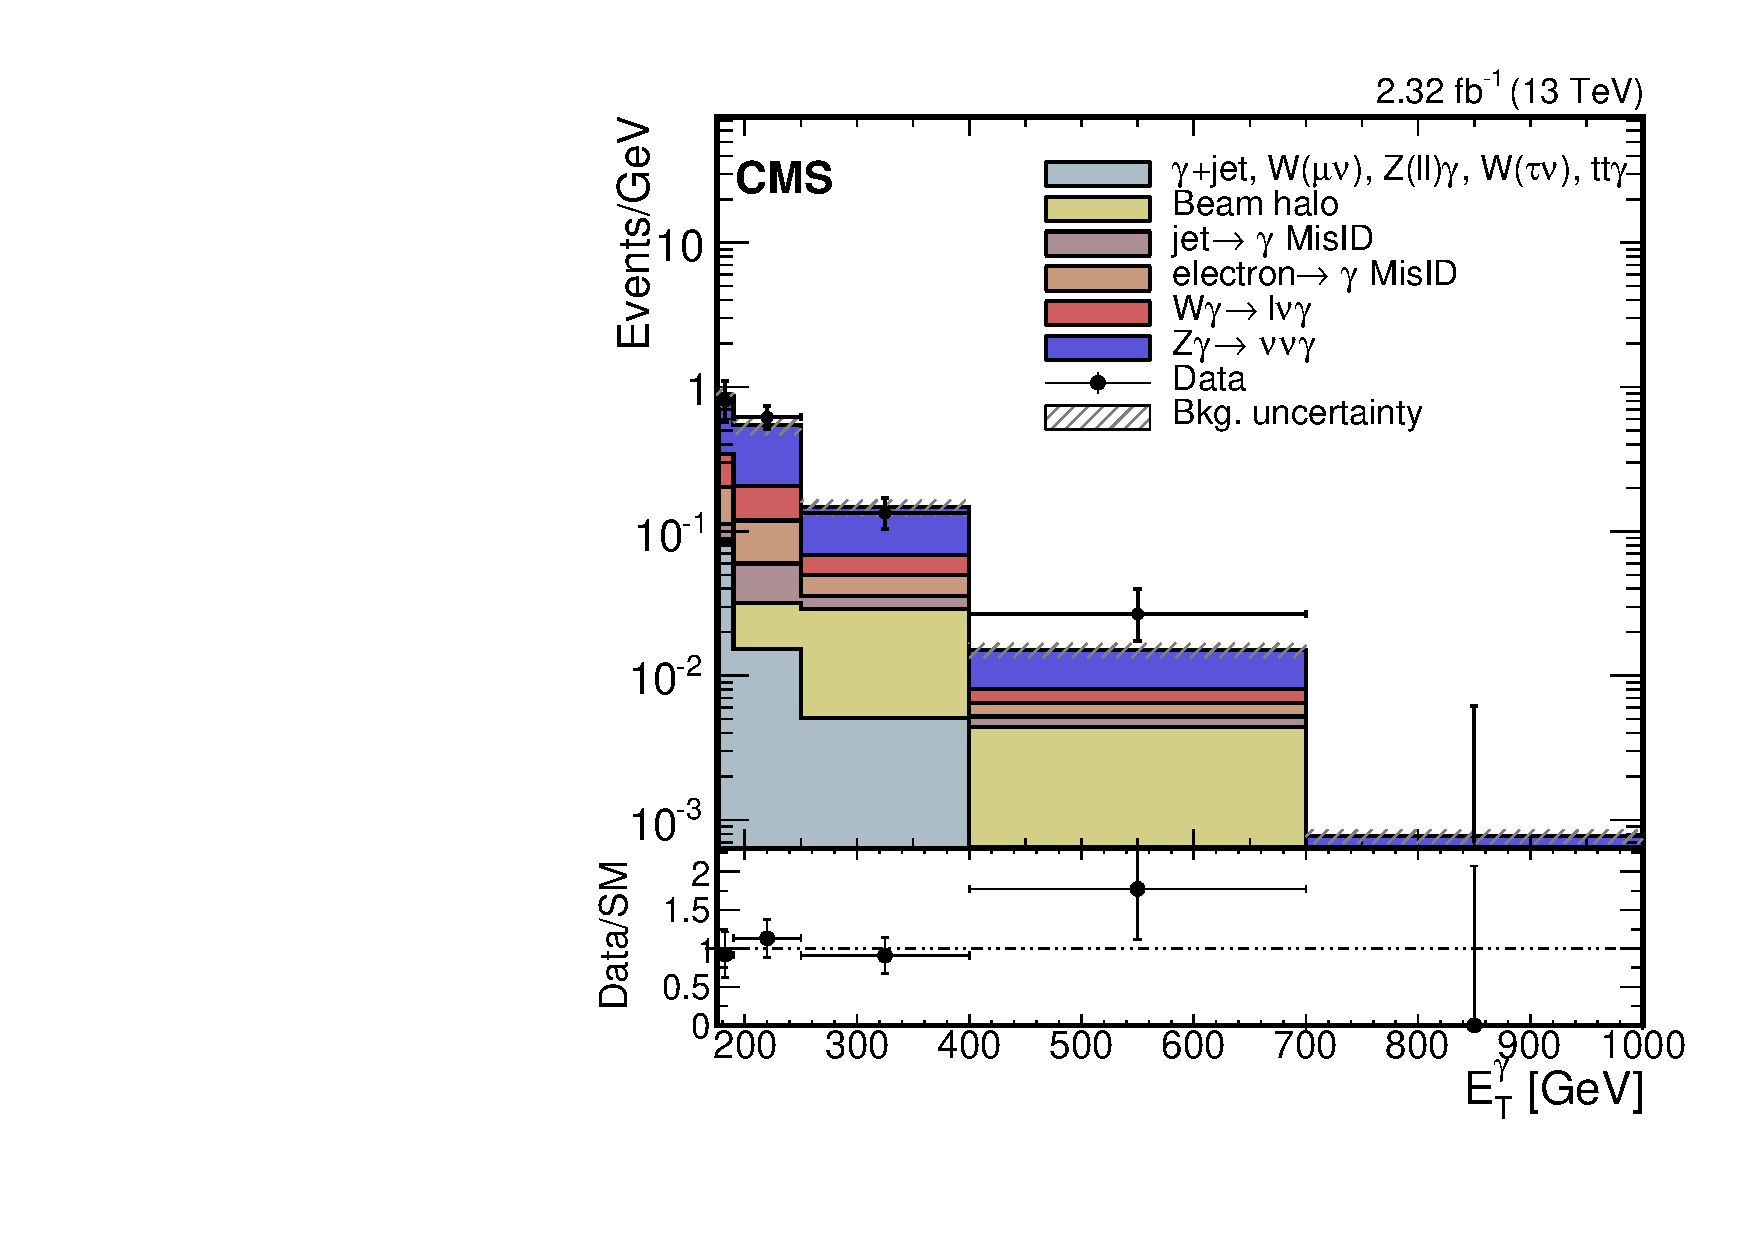
\includegraphics[width=8cm,height=8.0cm]{/Users/rhombus/CMS/Thesis/thesis/pdfs/lgxc/fromb/photon_pt8.pdf}
%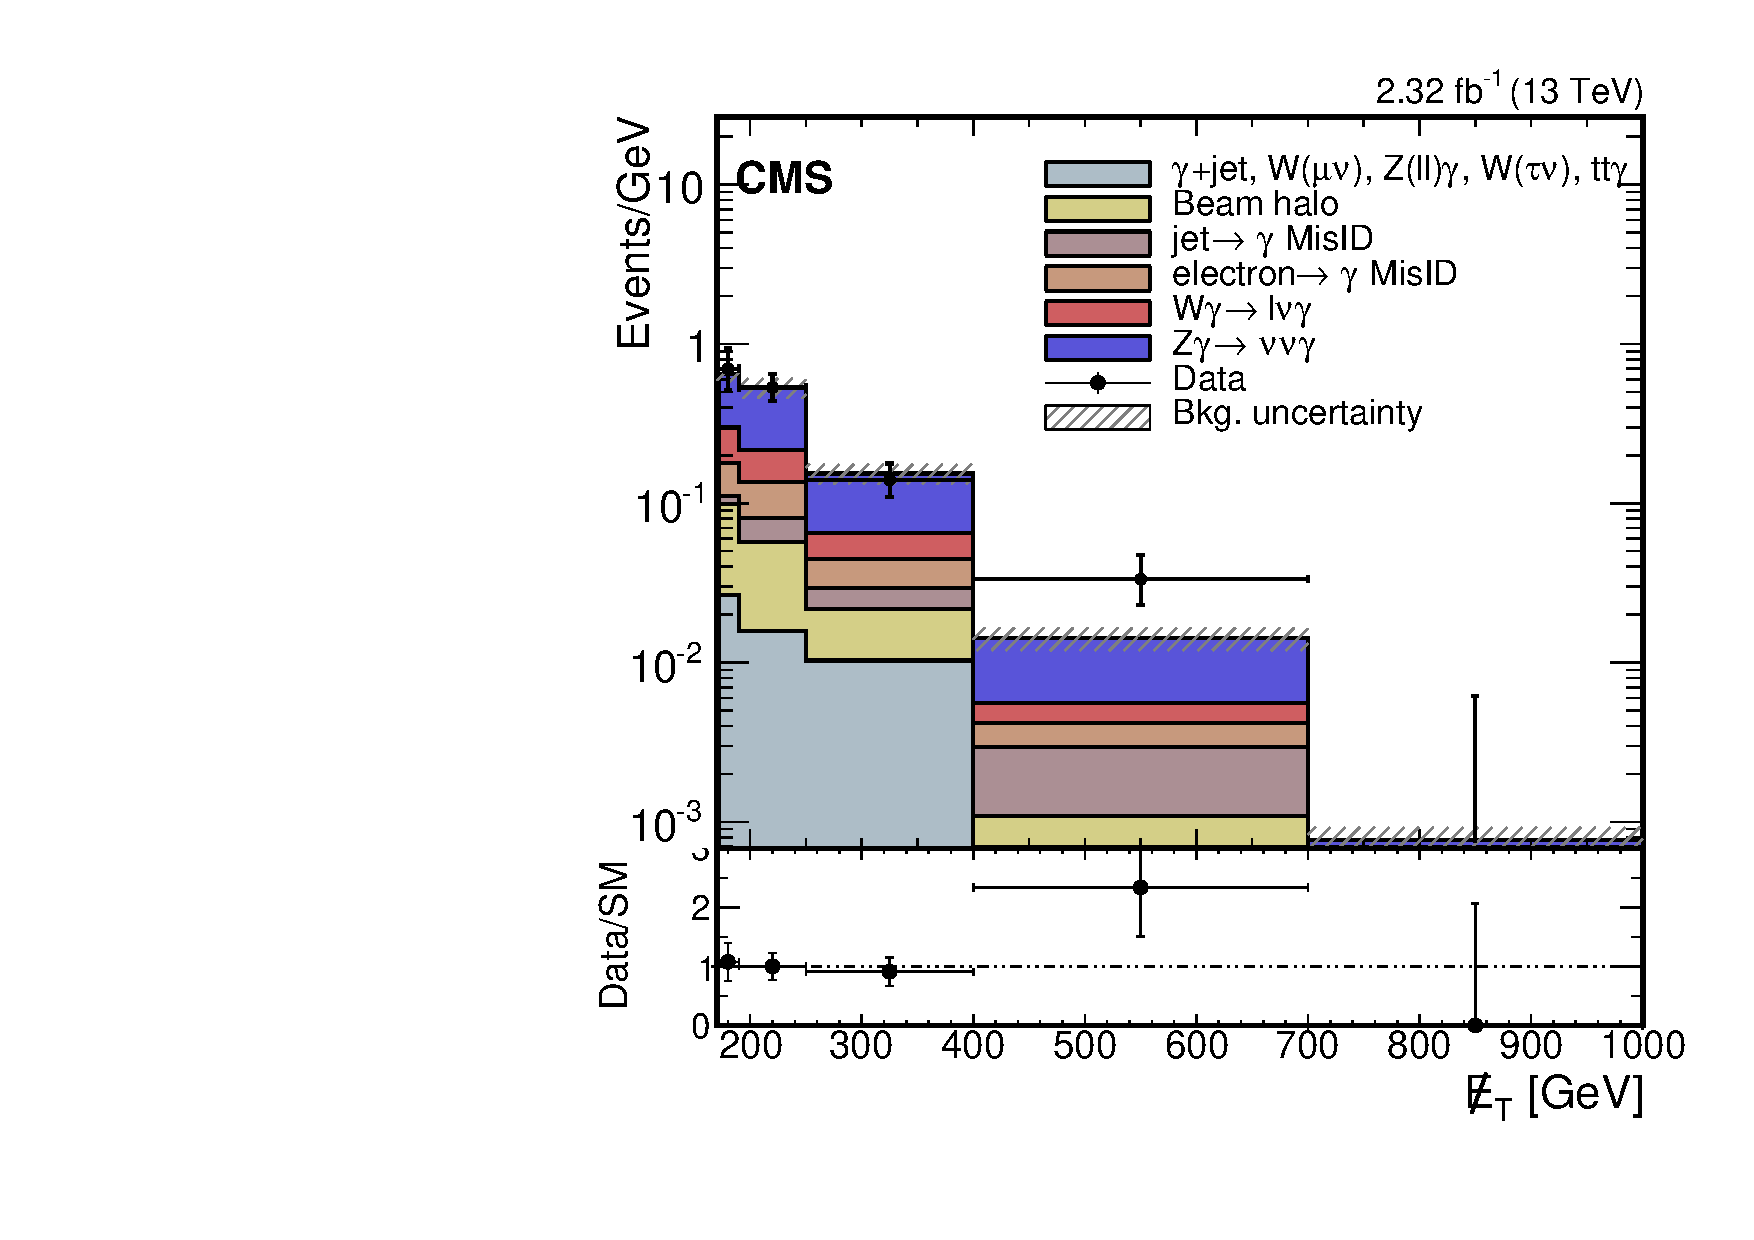
\includegraphics[width=8cm,height=8.0cm]{/Users/rhombus/CMS/Thesis/thesis/pdfs/lgxc/fromb/met8.pdf}
%\label{fig:ptmetstack}
%\end{figure}

 \subsection{\vg Estimates}
After accounting for the event selection efficiency difference between data and MC,
 respectively $42.1 \pm 6.3$ and $10.7 \pm 1.5$ events are estimated
 from \zgnng\ and \wglng. 
Four sources of systematic uncertainty on \zg and \wg estimates are considered:
PDF and scale uncertainties are
 found using the the LHAPDF/PDF4LHC recommendations
 of varying the scales up and down by a factor of 2 
 and using PDf sets from CTEQ, MSTW and NNPDF 
 to be 5.37\% and 8.9\% respectively.
Electroweak correction uncertainties
 are estimated conservatively as the quoted uncertainties
 which are 11\% for \zg and 7\% for \wg.
Scale factors are estimated to have an uncertainty of 6\%
 which mostly  arises from the statistical limitations of the data samples
 used.
The sytematic uncertainty due to jet/\met/$\gamma$
 energy scale and pileup, is estimated at 6.2\%
 by shifting the energy of the respective PF object
 and observing the relative change in the number
 of events passing selections.  
%To gain confidence in the estimates from simulation, control regions
% dominated by the various backgrounds and having negligible
% contributions from the signal, are defined in the data. 
As a crosscheck, the total contribution from \zgnng is estimated
 in data using a sample of \zgllg candidates,
 where the leptons from the decay of the Z boson are removed and considered as
 \met~\cite{monojet2014}. 
This provides an estimate of $64.6 \pm 17.6$, 
 where the uncertainty is dominated by the size of the sample.

 \subsection{Elecron Mis-ID}
The most important SM background comes from events where
 electrons are misidentified as photons, mainly in the \wen process. 
Seeding efficiency in the pixel detector for
 electron tracks is $\epsilon = 0.982 \pm 0.004$ for
 electrons with $\pt > 100\GeV$. 
This efficiency is measured in data using the
 tag-and-probe method~\cite{Khachatryan:2010xn} on \zee events,
 and is verified with MC simulation. 
Electrons from \w\ boson decay that are not seeded
 appear as isolated photons accompanied with large \met from the escaping neutrino. 
This class of events is modeled by an electron proxy event sample
 selected in data using criteria that are identical to those described in 
 Sec.~\ref{subsec:lgevent_selection}, except the photon candidate is required to have
a pixel seed. 
The number of electron proxy events is then scaled by
 $(1-\epsilon)/\epsilon$ where $\epsilon$ is the efficiency
 to yield an estimated contribution of $7.4 \pm 1.2$ from
 electron misidentification events. 
The dominant uncertainty in the 
 estimate is the statistical uncertainty in the tag-and-probe fit, 
 and is assessed by generating a large ensemble
 of toy dielectron mass distributions
 on which the fit procedure is repeated. 
The standard deviation of the number
 of \zee events obtained from the fits is then propagated
 to the uncertainty in the efficiency.

 \subsection{Non-collision Backgrounds}
Non-collision backgrounds,  from  things such as detector noise,
 cosmic rays, and beam halo, are estimated from the time distribution of the cluster seeds
 since each process exhibits a disctintive time distribution when the cluster is
 in the ECAL barrel. 
Templates for anomalous signals, cosmic ray muons, and beam halo events
 are obtained by inverting the shower shape and beam halo tag requirements,
 and are fitted to the timing distribution of the candidate sample.
The only nonnegligible residual contribution to the candidate sample
 is found to arise from the beam halo, with an estimated $5.9\pm4.7$ events
 coming directly from the template fit.
%As a cross-check, a fit to the azimuthal angle ($\phi$) distribution of the candidate
% sample is performed. 
%Beam halo EM showers are observed to concentrate around
%$\phi \sim 0,\pi$, while all other (collision-origin) processes should yield
%photons that are uniformly distributed in $\phi$. This cross-check estimates
%the number of beam halo events in the signal sample to be less than 4.4 at 95\%
%confidence level.

 \subsection{Minor SM Processes}
The SM processes \wlng, \zllg, $W(l\nu)$ and $\gamma+jets$
 are generated with \MADGRAPH{}5$\_aMC@NLO$ at LO~\cite{Madgraph_new}
 with up to 2 jets and then
 processed with \PYTHIA6.426 generator~\cite{Pythia6} for showering and hadronization,
 with the \NNPDFthree LO($\as = 0.130$) parton distribution function.
The total background expectation from these processes is $3.05\pm 0.67$ events,
 where the uncertainty includes the statistical and systematic uncertainty due
 to scale factor and jet/\met/$\gamma$ energy scale.


 
\section{Results}

After applying the full selection criteria,
 77 events in 2.32 fb$^{-1}$ of data remain.
Table~\ref{tab:BkgSummaryC}
shows the estimated number of events and uncertainty from each background for the full 2015 run.
The \pt spectrum and PF \met of the full
 combination of selected candidate events and
 estimated backgrounds can be seen in Figure \ref{fig:ptmetstack}
 along with distributions of \pt/\met and 
 the number of jets.
%Likewise, Figure~\ref{fig:ratio_stack} and Figure~\ref{fig:addplots} shows the jet \pt, nvertices and $E_{T}^{\gamma}$/\met, $E_{T}^{\gamma}$/ jet \pt  for our selected candidate events and estimated backgrounds for the full candidate selection.
%Since data are compatible with the standard model expectation, upper limits on new physics processes cross
%sections are set.

\begin{figure}[htb]
\caption[Signal region distributions in the \pploneg analysis]
 {The photon \pt and \met\ distribution for the candidate sample,
  compared with estimated contributions from SM backgrounds are shown.
% on top
%  and the photon \pt/\met\ and number of jets distribution for the candidate sample
%  are shown below.
  Here QCD$\gamma$ refers to $\gamma$+jet background and the
  background uncertainity includes statistical and systematic error. }
\begin{centering}
\begin{tabular}{cc}
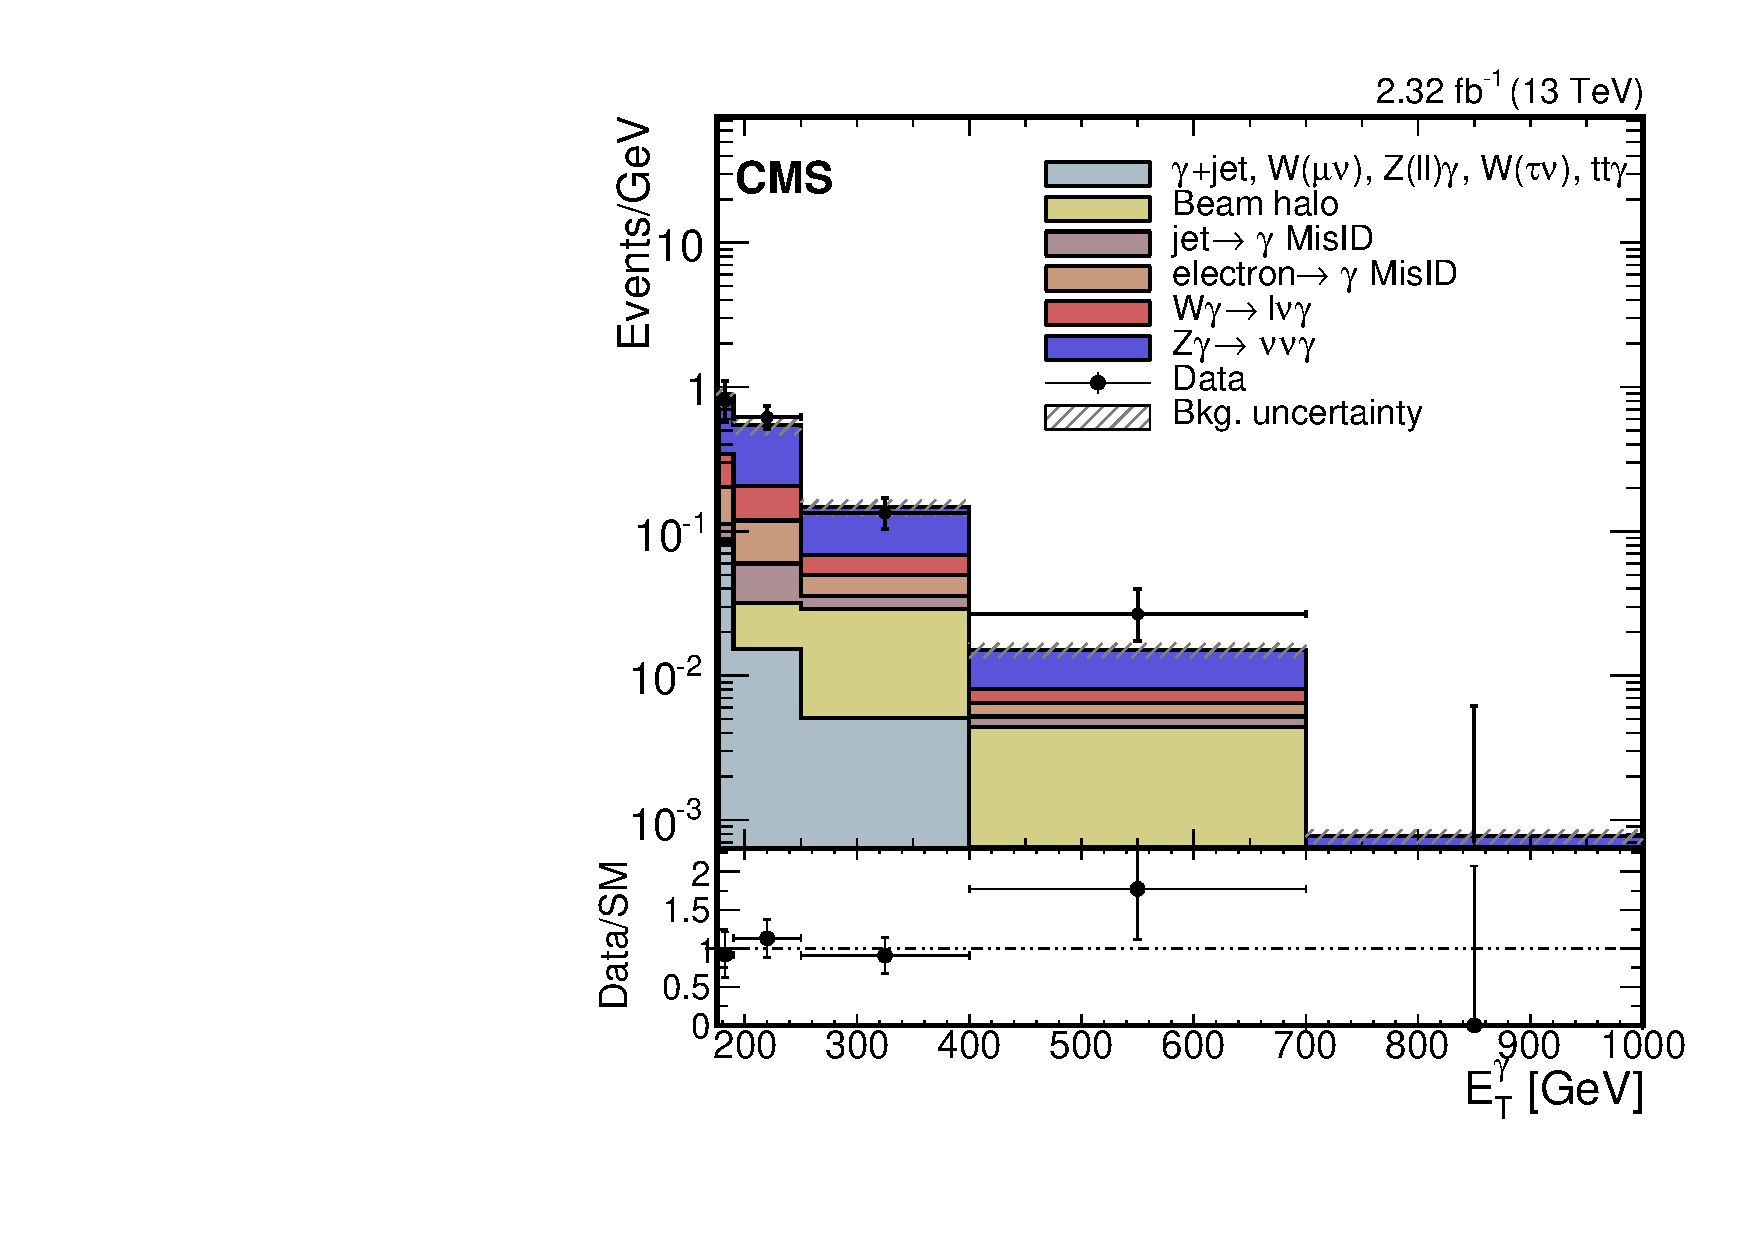
\includegraphics[width=0.4\textwidth]{/Users/rhombus/CMS/Thesis/thesis/pdfs/lgxc/fromb/photon_pt8.pdf} &
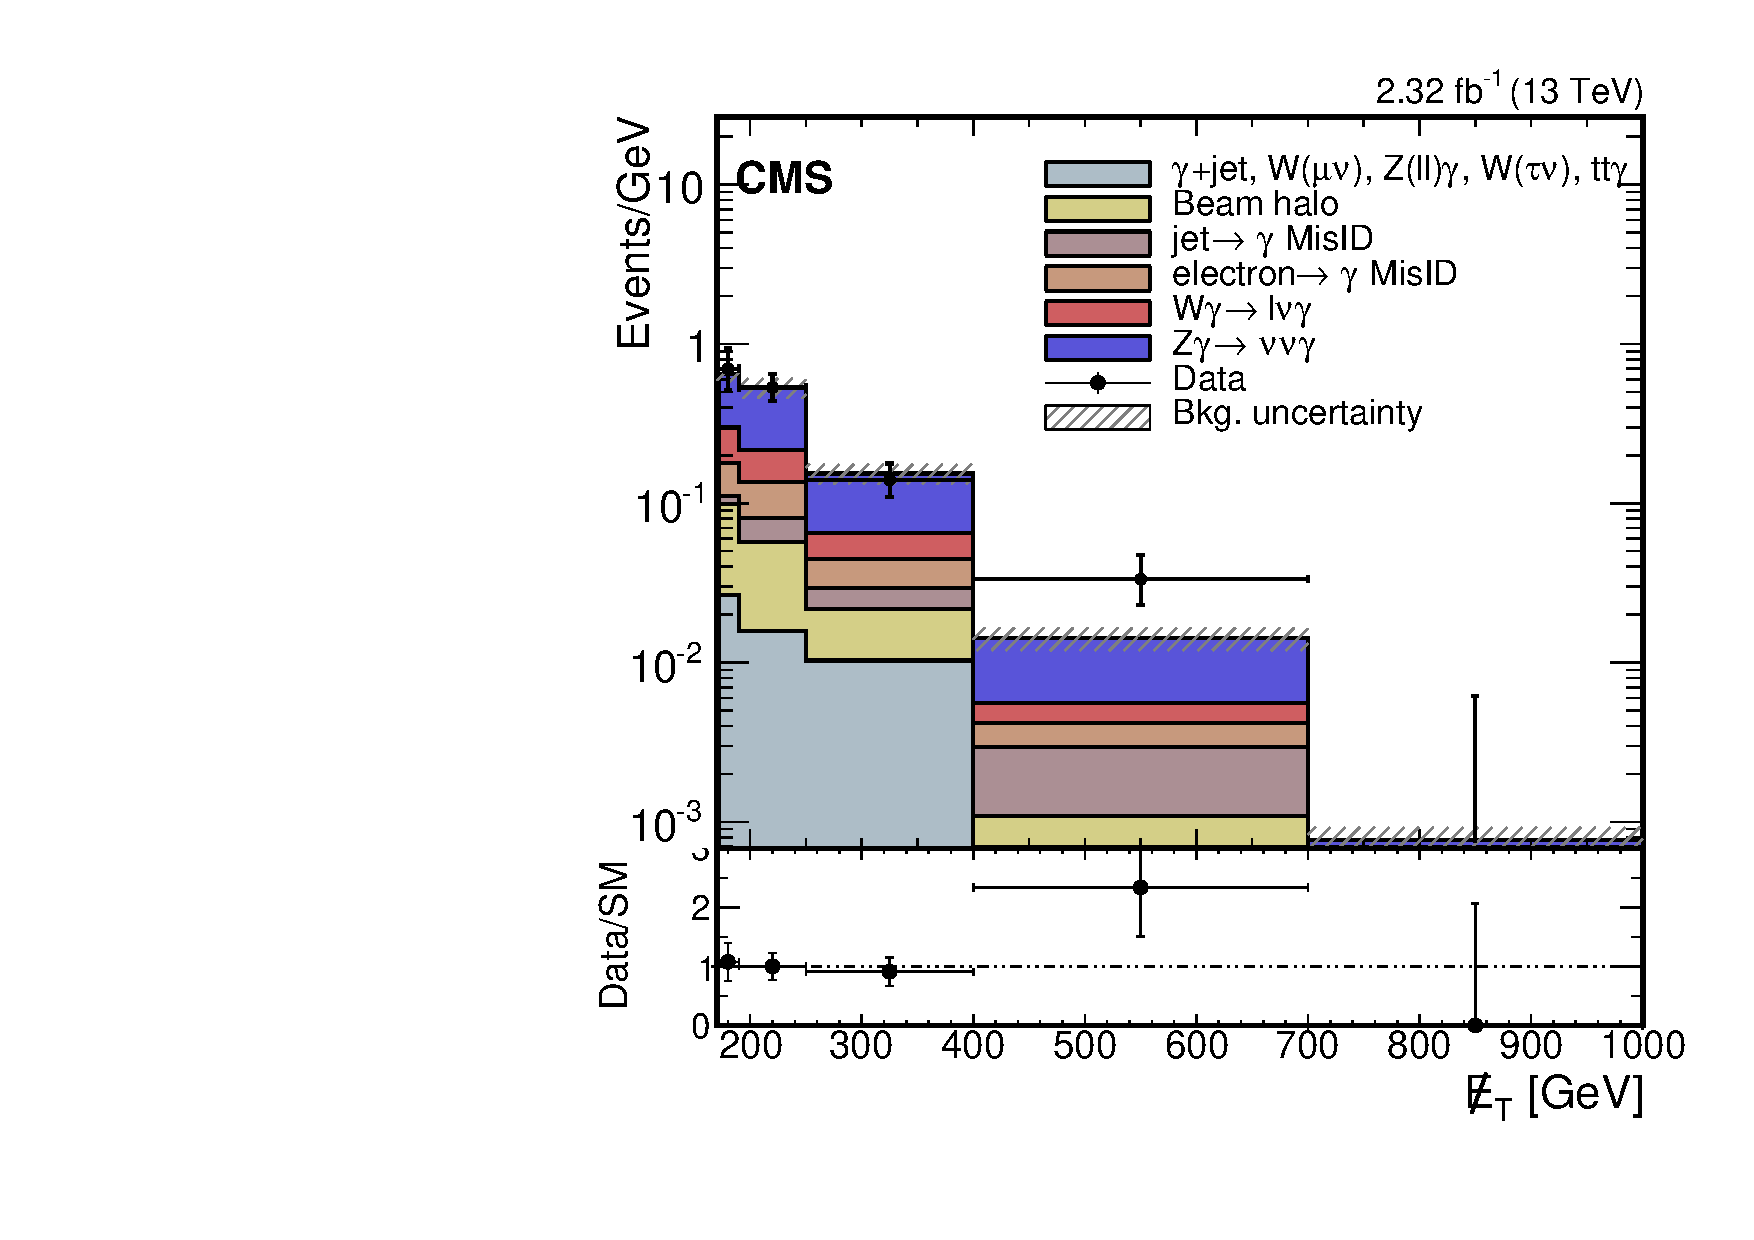
\includegraphics[width=0.4\textwidth]{/Users/rhombus/CMS/Thesis/thesis/pdfs/lgxc/fromb/met8.pdf}
%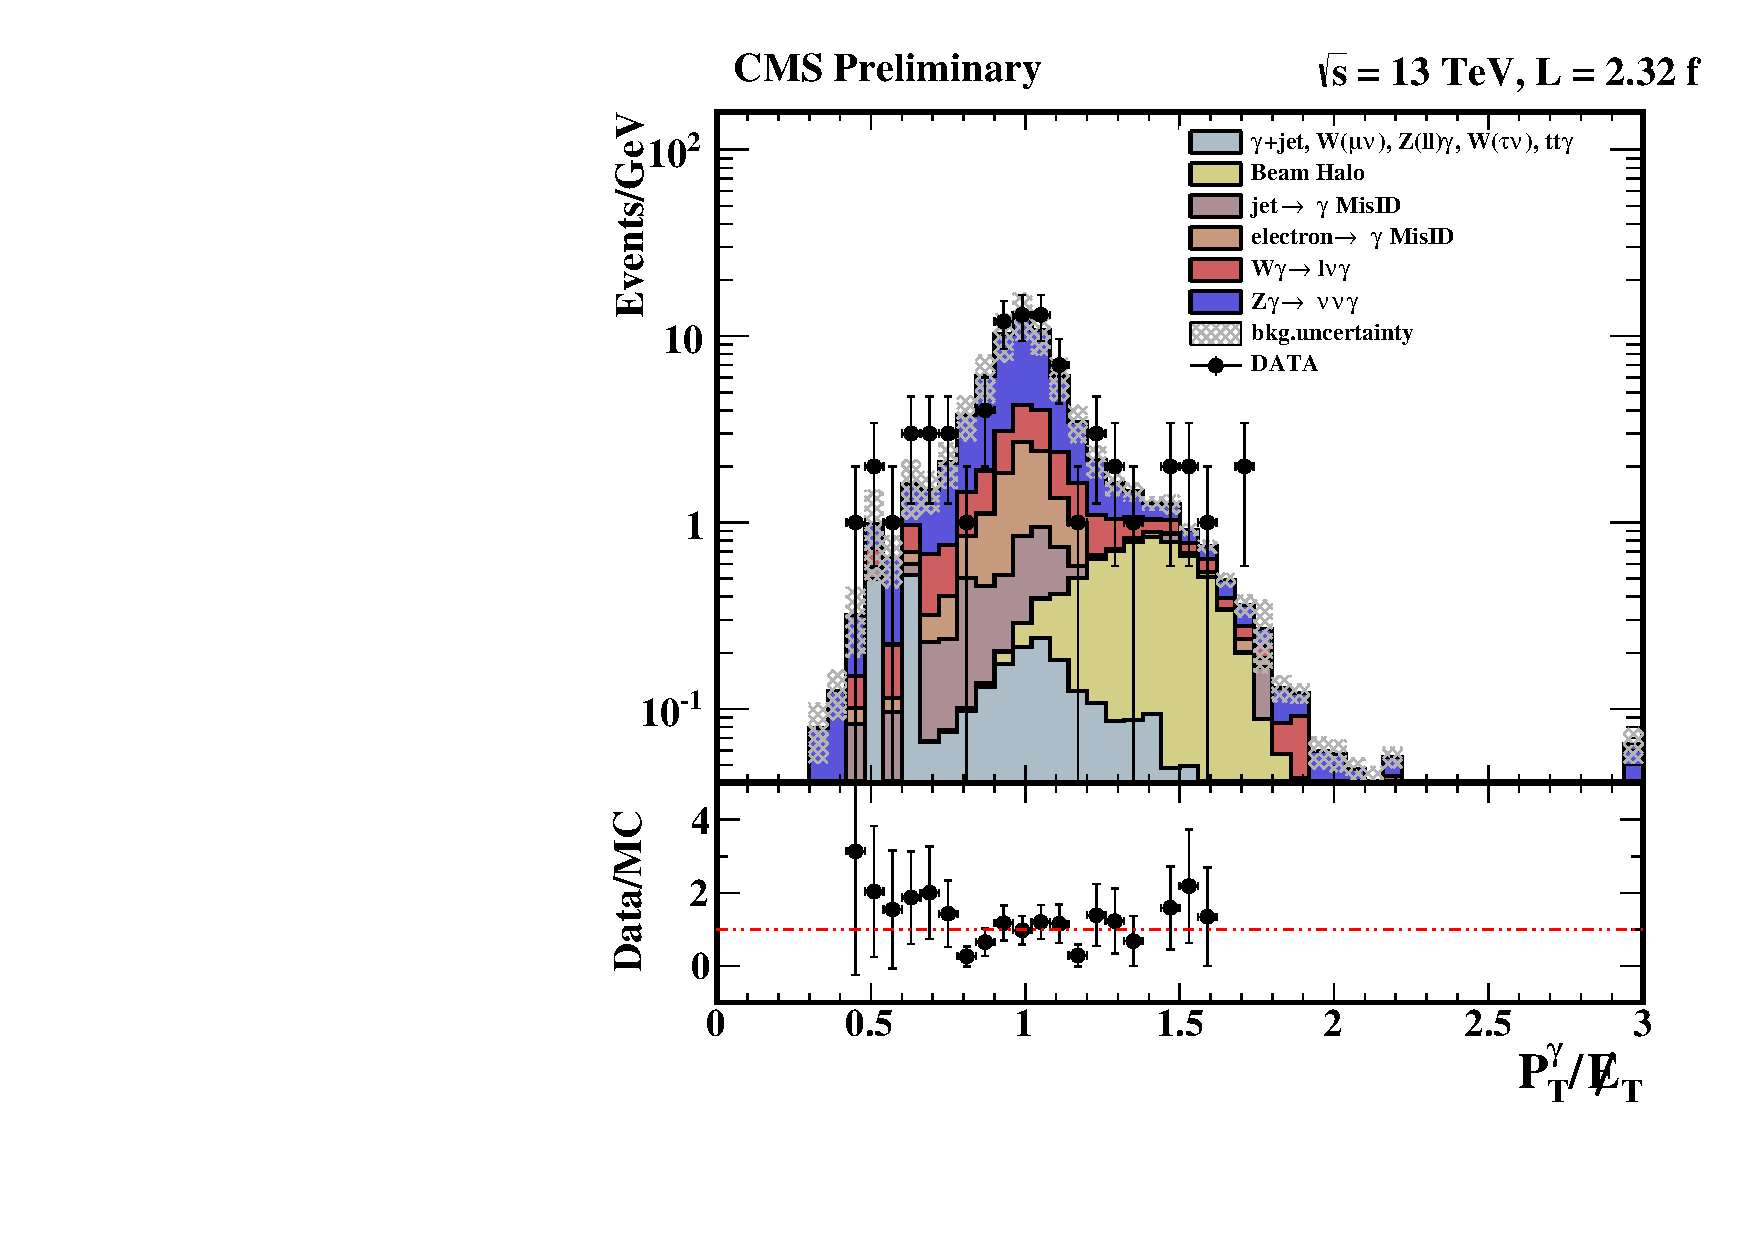
\includegraphics[width=0.4\textwidth]{/Users/rhombus/CMS/Thesis/thesis/pdfs/lgxc/fromb/ptmet8_err.pdf} &
%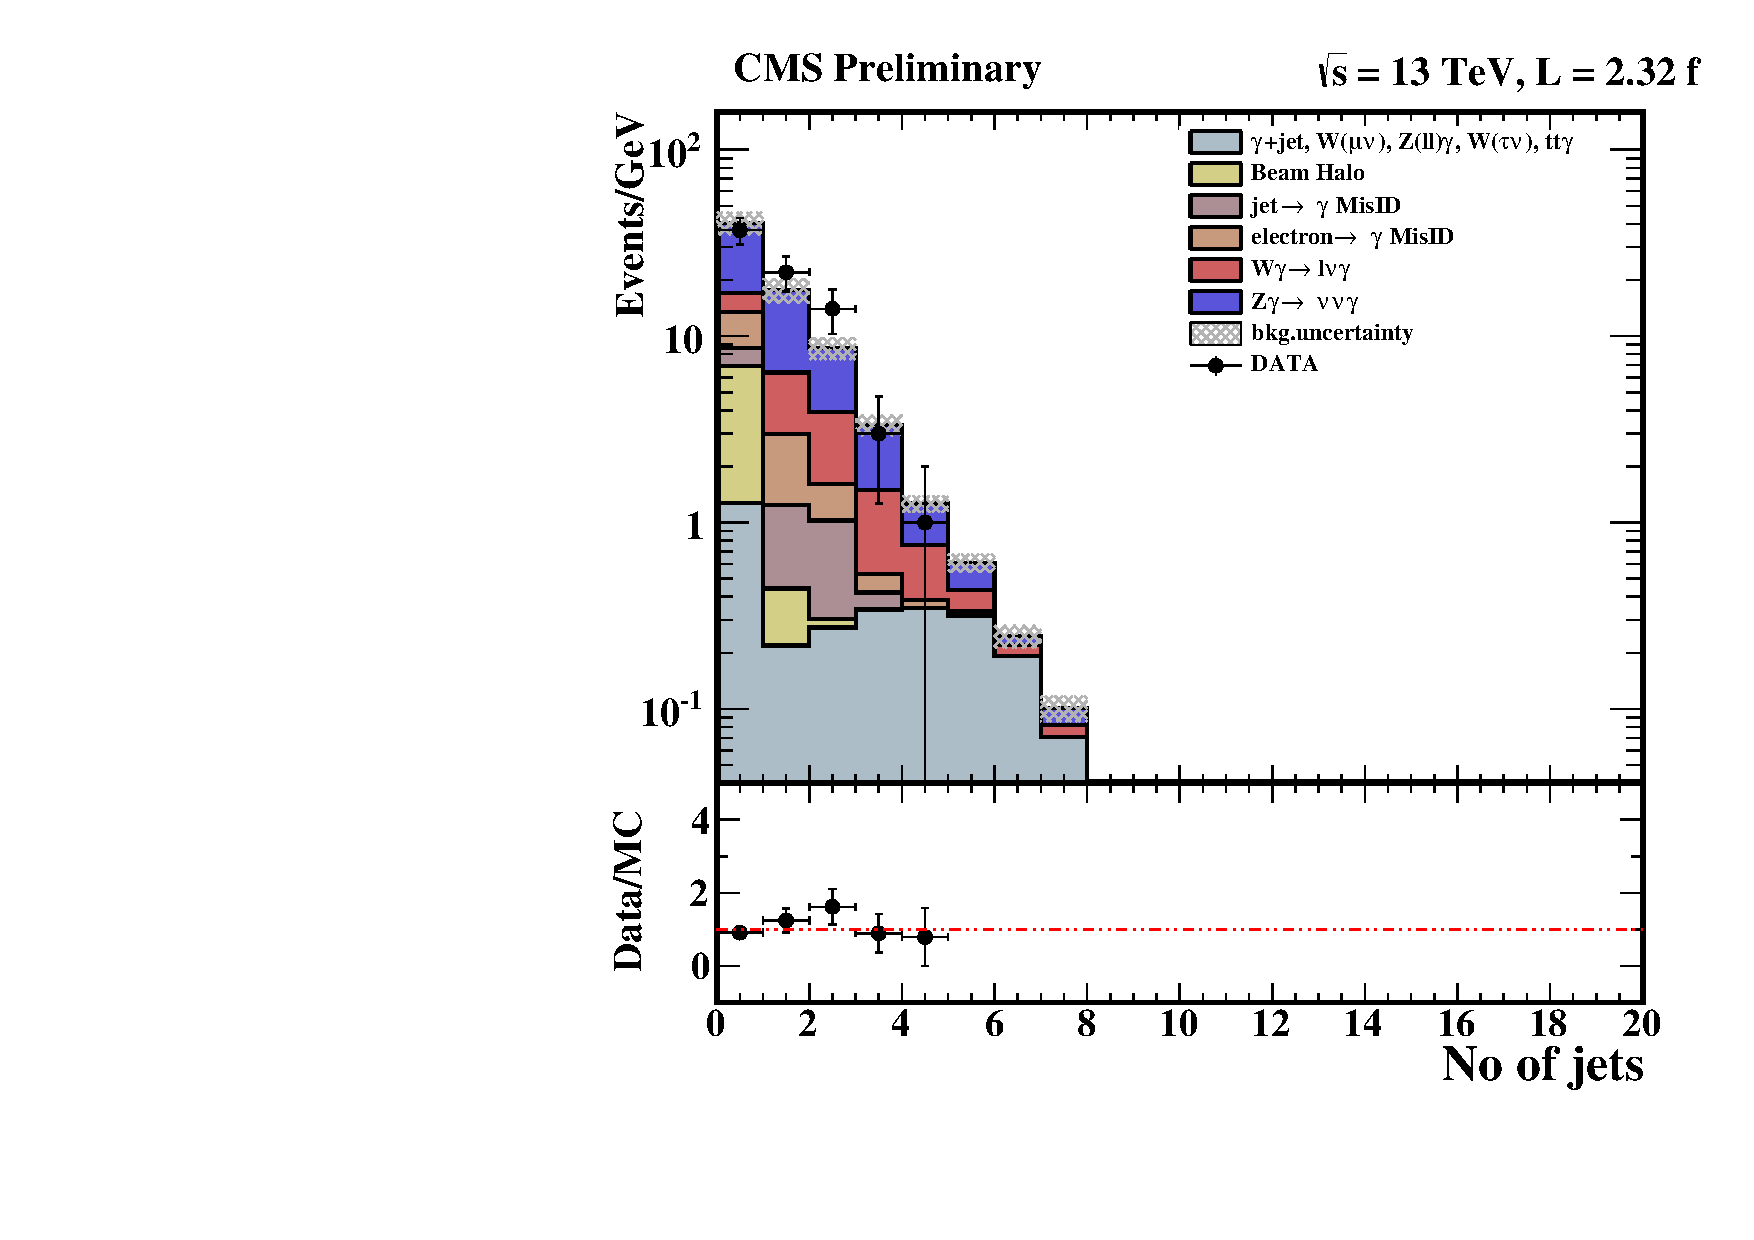
\includegraphics[width=0.4\textwidth]{/Users/rhombus/CMS/Thesis/thesis/pdfs/lgxc/fromb/njet30_err_withdphi.pdf}
\end{tabular}
\end{centering}
\label{fig:ptmetstack}
\end{figure}


%\begin{table}[htbp]
\begin{table}[!htb]
\caption[Estimated yields for \pploneg]
{
 Summary of estimated backgrounds and observed total number of candidates for 2.32 fb$^{-1}$ of 2015 data.
 The category Others includes \wmn, \zllg and \ttg
}
\center
{
\begin{tabular}{c|c}
Process & Estimate \\
\hline
\hline
\zgnng         & 42.10 $\pm$ 6.31   \\
\wglng         & 10.69 $\pm$ 1.49   \\
\wen           & 7.80  $\pm$ 1.78   \\
${jet}\rightarrow\gamma~{fakes}$ & 3.36$\pm$ 1.13 \\
Beam halo      &  5.9 $\pm$  4.7 \\
Others         & 3.05 $\pm$ 0.67  \\
\hline
Total Expectation  &  72.9 $\pm$ 8.30 \\
\hline
Data               & 77    \\
\end{tabular}
\label{tab:BkgSummaryC}
}
\end{table}

\subsection[\ppzgnng Cross Section Measurement]
{${\boldsymbol{\ppzgnng}}$ Cross Section Measurement}

The  \ppzgnng cross section for $\ptg >175$ \GeV in the
 range $\abs{\eta} <$ 1.4 is calculated using the formula

\begin{equation}
 \sigma(\ppzgnng) = \frac{N_{data}-N_{BG}}{A\times\epsilon\times L}
\end{equation}
 where $N_{data}$ is the observed number of events, 
 $N_{BG}$ is the number of estimated background events,
 $A$ is the geometrical and kinematic acceptance of the selection criteria,
 $\epsilon$ is the selection efficiency within the acceptance,
 and $L$ is the integrated luminosity.
%$Br$ is the branching ratio, which in this case is 100\%.
The product of $A\times\epsilon_{MC}$ is estimated from LO \MADGRAPH simulation and a
 correction factor, $\rho$, described in Section \ref{subsubsec:lg_reweighting}
 is applied to account for the difference between the efficiency in the data and 
 Monte Carlo:

\begin{equation}
 A\times\epsilon = A\times\epsilon_{MC} \times \rho  .
\end{equation}

The product of $A\times\epsilon_{MC}$ is estimated to be
 0.314 $\pm$ 0.002 (stat) $\pm$ 0.048 (syst) and rho is 0.99 $\pm$ 0.06.
%Here $A\times\epsilon$ is defined as the ratio of number of events
% passing the full selection to the number of events
% passing  \ptg$ > 175$ \GeV and $\abs{\eta} < 1.4442$.

% and the syst is 7 pecen scale and 6.2 photon/met gives 9%. syst of A*eff 0.0286

The photon energy scale, jet and \met energy scale and resolution,
 and pileup related contributions are considered as
 sources of systematic uncertainty in the acceptance calculation.
The uncertainty on the photon energy scale is about $1.5\%$
 and the uncertainty from variations in the \met energy scales is 5\%.
 %Uncertainties on $\met$ are estimated in accordance to the MET 
 %POG prescription~\cite{met}. 
Contributions from the jet energy scale are accounted for in the  uncertainty on  
the \met. 
The uncertainty on the integrated luminosity is 2.7$\%$~\cite{LUM-13-001}.
A summary of the systematic uncertainties are shown in Table ~\ref{tab:sysfull1}.

\begin{table}[htbp]
\caption[Systematic uncertainties in \pploneg]{Summary of systematic unceratinties for signal and different background sources.}
\centering
%{\scriptsize
\resizebox {\textwidth }{!}{ % 
\begin{tabular}{c|c|c|c|c|c|c}
Sources & \zgnng [\%] & \wglng [\%] & $j$ faking $\gamma$ [\%] & $e$ faking $\gamma$ & $\gamma j$ & Other bkgs [\%] \\
\hline
\hline
Luminosity & 2.7    & 2.7  & - & - & 2.7 &  2.7 \\
\hline
PDF and Scale & 5.37 & 8.9 & - & -& -& -\\ 
\hline
EWK corrections &  11 & 7 & - & - & - & -\\ 
\hline
$j$ faking $\gamma$ & - & - & 30 & - & - & -\\ 
\hline
$e$ faking $\gamma$ & - & -& -& 20 & - & -\\ 
\hline
$j$,\met,$\gamma$ energy scale &  6 & 6 &-& - & 6 & 6\\ 
\hline
Scale Factors & 6 & 6 & -& - & 6 & 6
\end{tabular}}
\label{tab:sysfull1}%}
\end{table}

The measured cross section for \ppzgnng  for photon $p_T >$ 175 GeV within
 rapidity range $\mid \eta_{\gamma}\mid < $1.4
 is 
\begin{equation}
 64.06 \pm 12.14(\mathrm{stat}) \pm 12.88(\mathrm{syst}) \pm 1.72(\mathrm{lumi})\;\; \fb.
\end{equation}
The NNLO therotical cross section is $65.55\pm 0.02$ \fb
  where the uncertainty includes only the scale variaitons. 
The measured cross section agrees well with the NNLO theoritical cross section
 and this agreement with the SM prediction constrains
 possible DM models.

 \subsection{Limits on Dark Matter}
\label{ssec:lim_DM}
Interpreting these results as setting limits on the
 cross section of a DM particle as a function of 
 DM mass, Tables~\ref{table:vxslimits} and \ref{table:avxslimits}
 show 90\% confidence level (CL) upper limits on the
 production cross sections provided infor the Vector
 and the Axial-vector model for a mediator mass of 10 \TeV. 
%Using a type-I error rate ($\alpha$) of 0.10 instead of the ``industry standard'' 0.05 used in exotic searches because we want to compare our results against other experiments for which $\alpha=0.10$ is considered standard.
%We are working on other mass points for the dark matter and will present results soon.


\begin{table}[ht]
\caption[Upper limits on DM cross section for vector $m_M = 10$ \TeV]
{Observed (expected) 90\%CL upper limits on the DM production cross section $\sigma$ for vector mediator mass 10 TeV. }
\centering
\begin{tabular}{cc}
\hline\hline
Mass DM [GeV] & $\sigma$ [fb] \\
\hline
1  & 3.821(3.242)  \\  
\hline
10  & 3.820(3.244)  \\  
\hline
50  & 3.827(3.249) \\
\hline
150  & 3.826(3.254)\\
\hline 
500  & 3.588(3.052) \\
\hline
1000  & 3.370(2.862) \\
\hline
\end{tabular}
\label{table:vxslimits}
\end{table}

\begin{table}[htb]
\caption[Upper limits on DM cross section for axial-vector $m_M = 10$ \TeV]{Observed (expected) 90\%CL upper limits on the DM production cross section $\sigma$ for axial vector  mediator mass of 10 \TeV }
\centering
\begin{tabular}{cc}
\hline\hline
Mass DM [GeV] & $\sigma$ [pb] \\
\hline
1  & 3.782(3.211)  \\  
\hline
10  & 3.785(3.213) \\
\hline
50  & 3.793(3.213) \\
\hline
150  & 3.754(3.192)\\
\hline
500  & 3.488(2.961)\\
\hline
1000  & 3.30(2.814)\\
\hline
\end{tabular}
\label{table:avxslimits}
\end{table}



Figure~\ref{fig:2d} shows the upper limits on the ratio of the cross section with respect
to the theoretical predictions ($\mu=
\sigma^{95\%}/\sigma_{Th}$) for the vector and axial-vector
mediator scenarios on the $m_\chi$-$m_M$ plane. The solid red and 
black curves are the expected and observed exclusion contours. The uncertainty on the 
expected upper limit includes the experimental uncertainties. For the simplified DM model
considered, a mediator mass of up to 600~\GeV is excluded for $m_\chi <10$ \GeV.

Exclusion contours in Figure~\ref{fig:2d} are also translated into the 
$m_\chi$-$\sigma_{SI/SD}$ plane as shown in Figure~\ref{fig:cont} where $\sigma_{SI/SD}$ are the 
spin-independent/dependent DM-nucleon scaterring cross sections~\cite{dmforum}. For 
these contours, we use 90\% CL to do a direct comparison
with the limits from the direct detection experiments~\cite{pico,pico1,lux1june}.

For DM EFT model with a contact interaction of type $\gamma\gamma\chi\overline{\chi}$, upper limits are placed on the production cross section, which are then translated into the lower limits on the suppression scale $\Lambda$. The 95\% CL observed and expected lower limits on $\Lambda$ as a function of dark matter mass $m_{\chi}$ are shown in Figure~\ref{fig:DMEWKlimits}. Values of $\Lambda$ up to 542\GeV are excluded at $95\%$ CL.

\begin{figure}[htb]
\caption[Exclusion plots in $m_{\chi}-m_M$ plane]{95\% CL upper limits on $\mu$= $\sigma$/$\sigma_{Th}$ in the $m_{\chi}$-$M_{M}$ plane for vector and axial-vector mediator, assuming couplings $g_{q}$ =0.25 and $g_{\chi}$ =1.
The The solid red and black curves are the expected and observed exclusion contours. 
The dotted black contours around the observed limit and the
 dotted red contours around the expected limit represent the
 one standard deviation theoretical uncertainties in the cross
 section and the combination of the statistical and experimental
 systematic uncertainties, respectively.}
\label{fig:2d}
\begin{center}
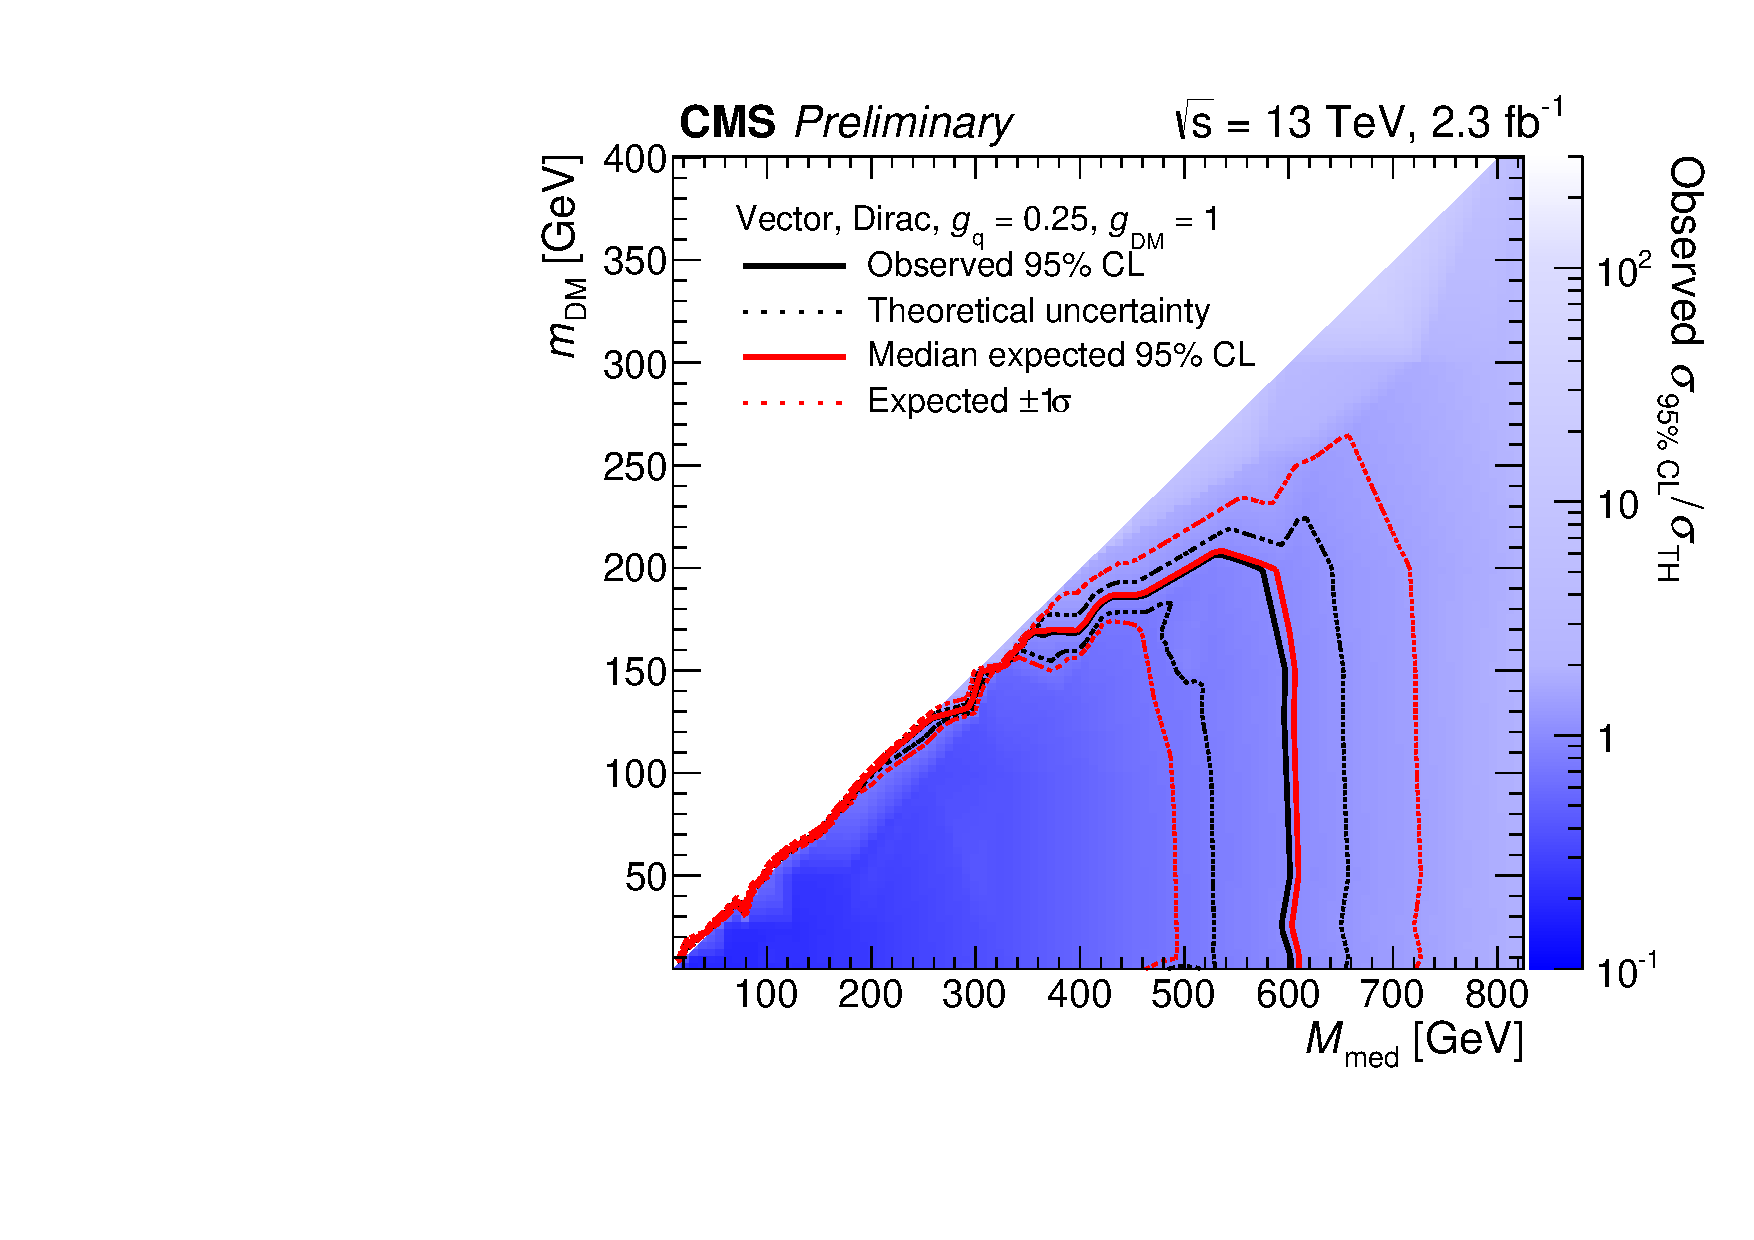
\includegraphics[width=0.4\textwidth]{pdfs/lgxc/fromb/V.pdf}
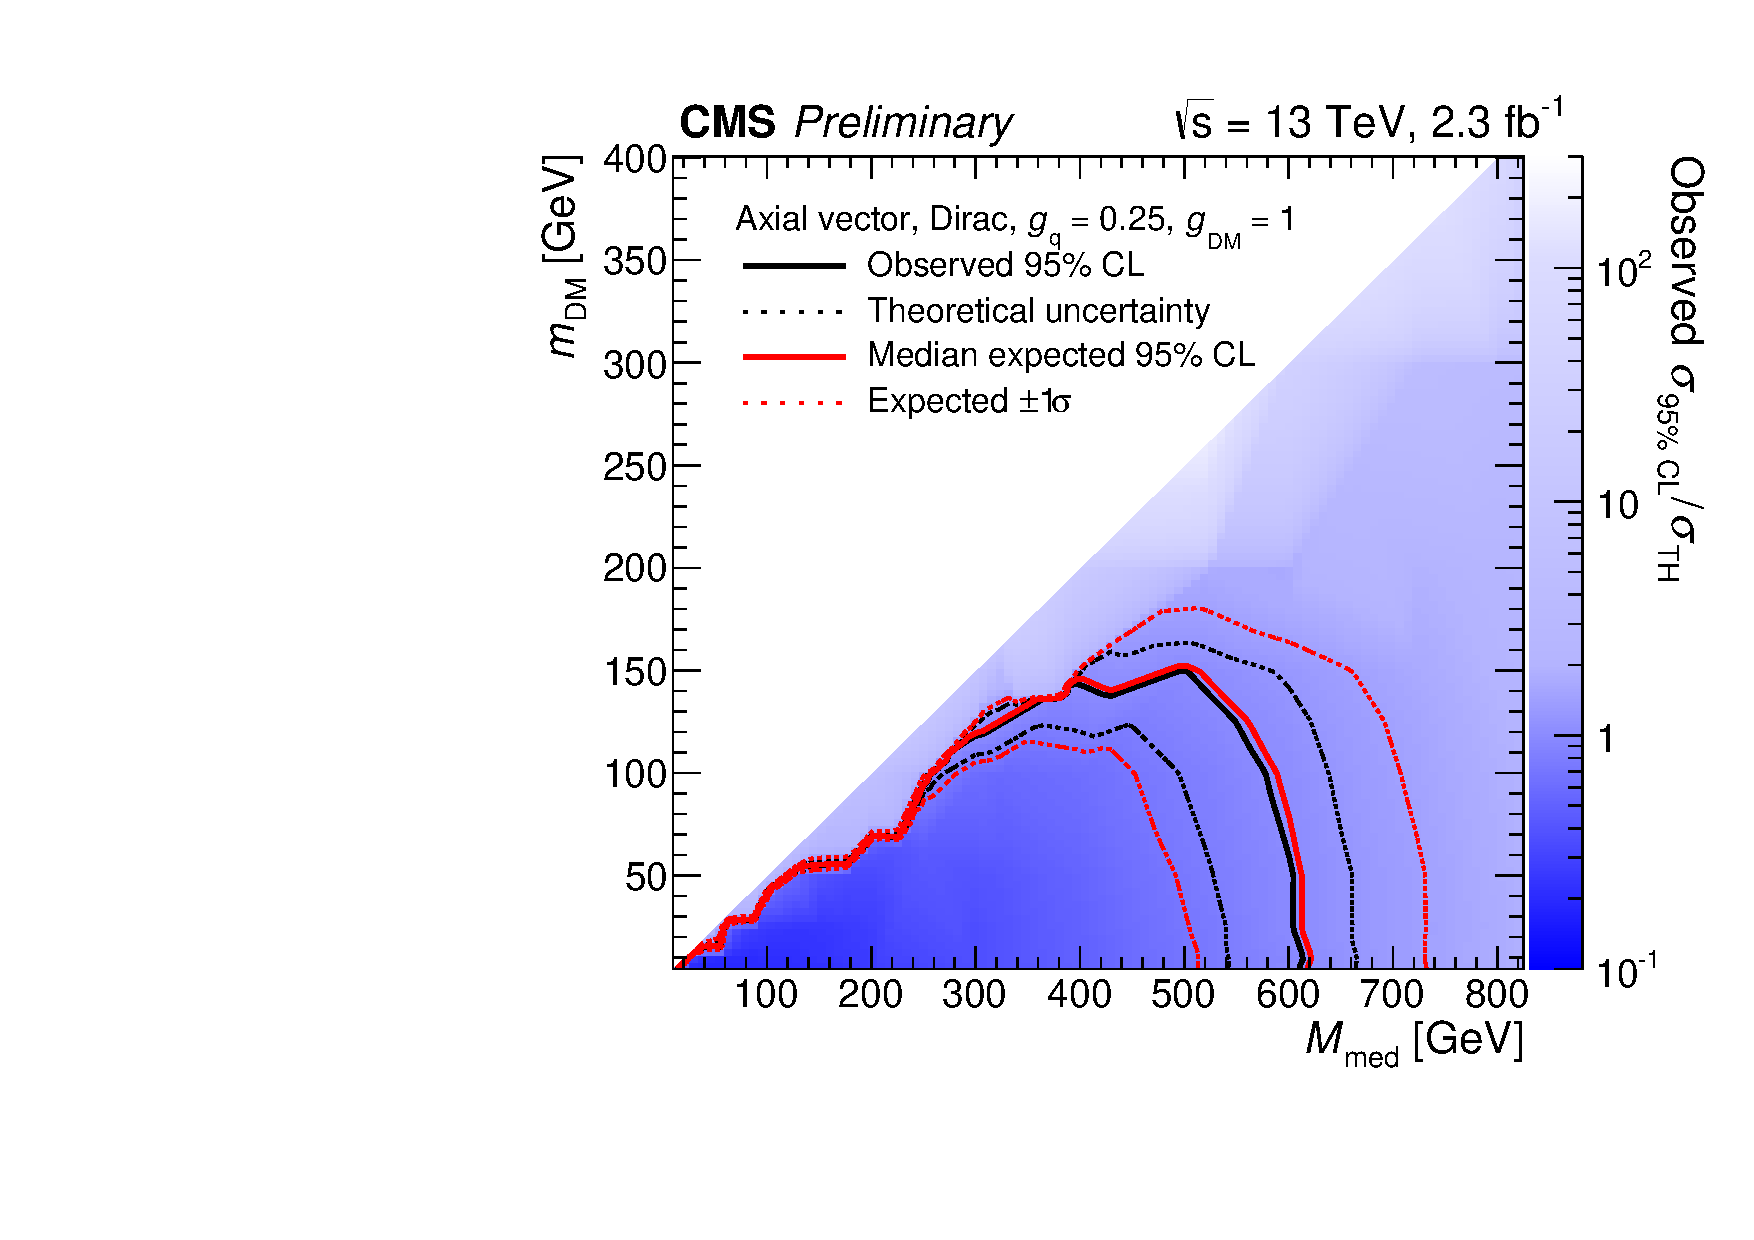
\includegraphics[width=0.4\textwidth]{pdfs/lgxc/fromb/AV.pdf}
\end{center}
\end{figure}

\begin{figure}[htb!]
\caption[Exclusion limits on DM-nucleon cross section]{The 90\% CL exclusion limits on the $\chi$-nucleon scattering cross section in a simplified model of dark matter production involving a vector and axial-vector operator as a function of the dark matter mass $m_{\chi}$.}\label{fig:cont}
\begin{center}
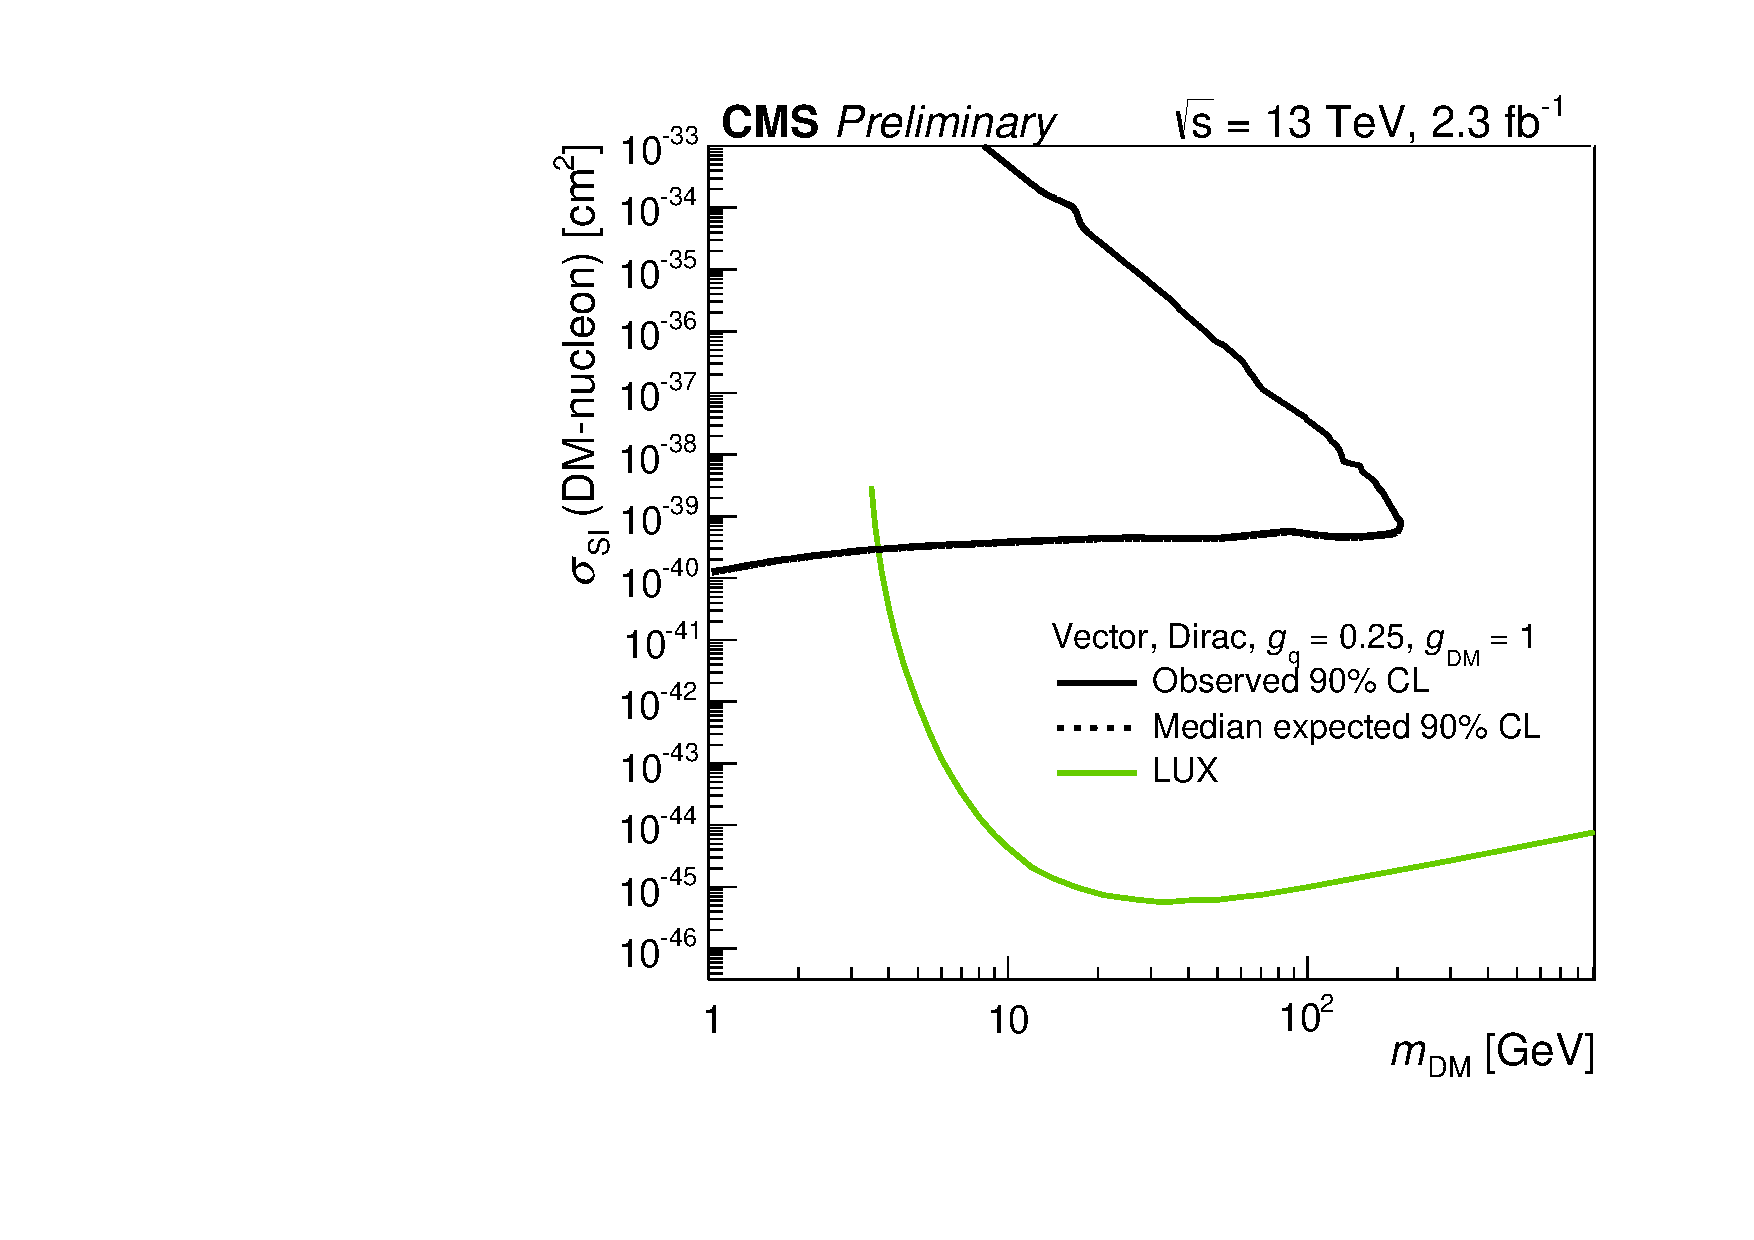
\includegraphics[width=0.4\textwidth]{pdfs/lgxc/fromb/SI.pdf}
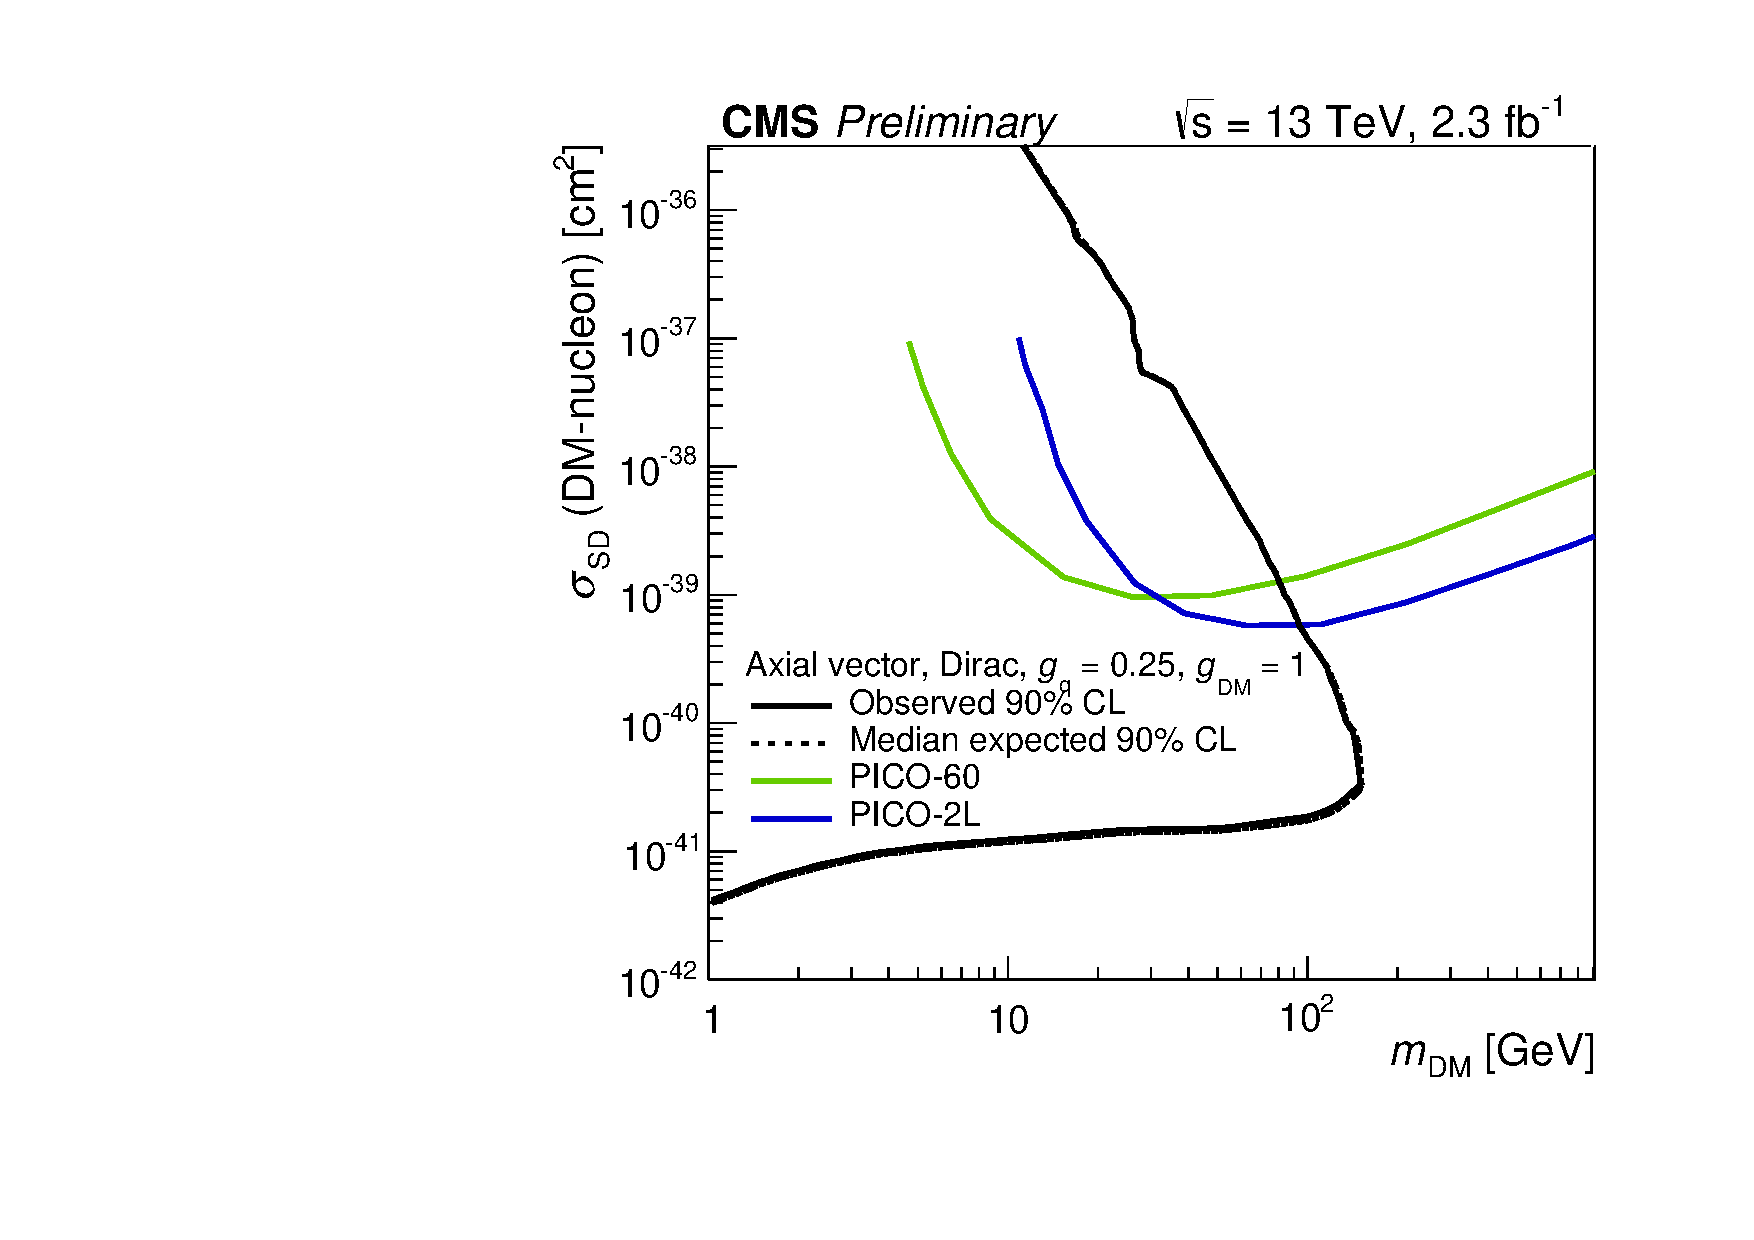
\includegraphics[width=0.4\textwidth]{pdfs/lgxc/fromb/SD.pdf}
\end{center}
\end{figure}

\begin{figure}[htb!]
\caption[Expected lower limit for EFT cutoff parameter $\Lambda$]{(a) The 95\% CL observed and expected lower limits on $\Lambda$ for a dimension-7 operator EFT model with a contact interaction of type $\gamma\gamma\chi\overline{\chi}$ as a function of dark matter mass $m_{\chi}$.}\label{fig:DMEWKlimits}
\begin{center}
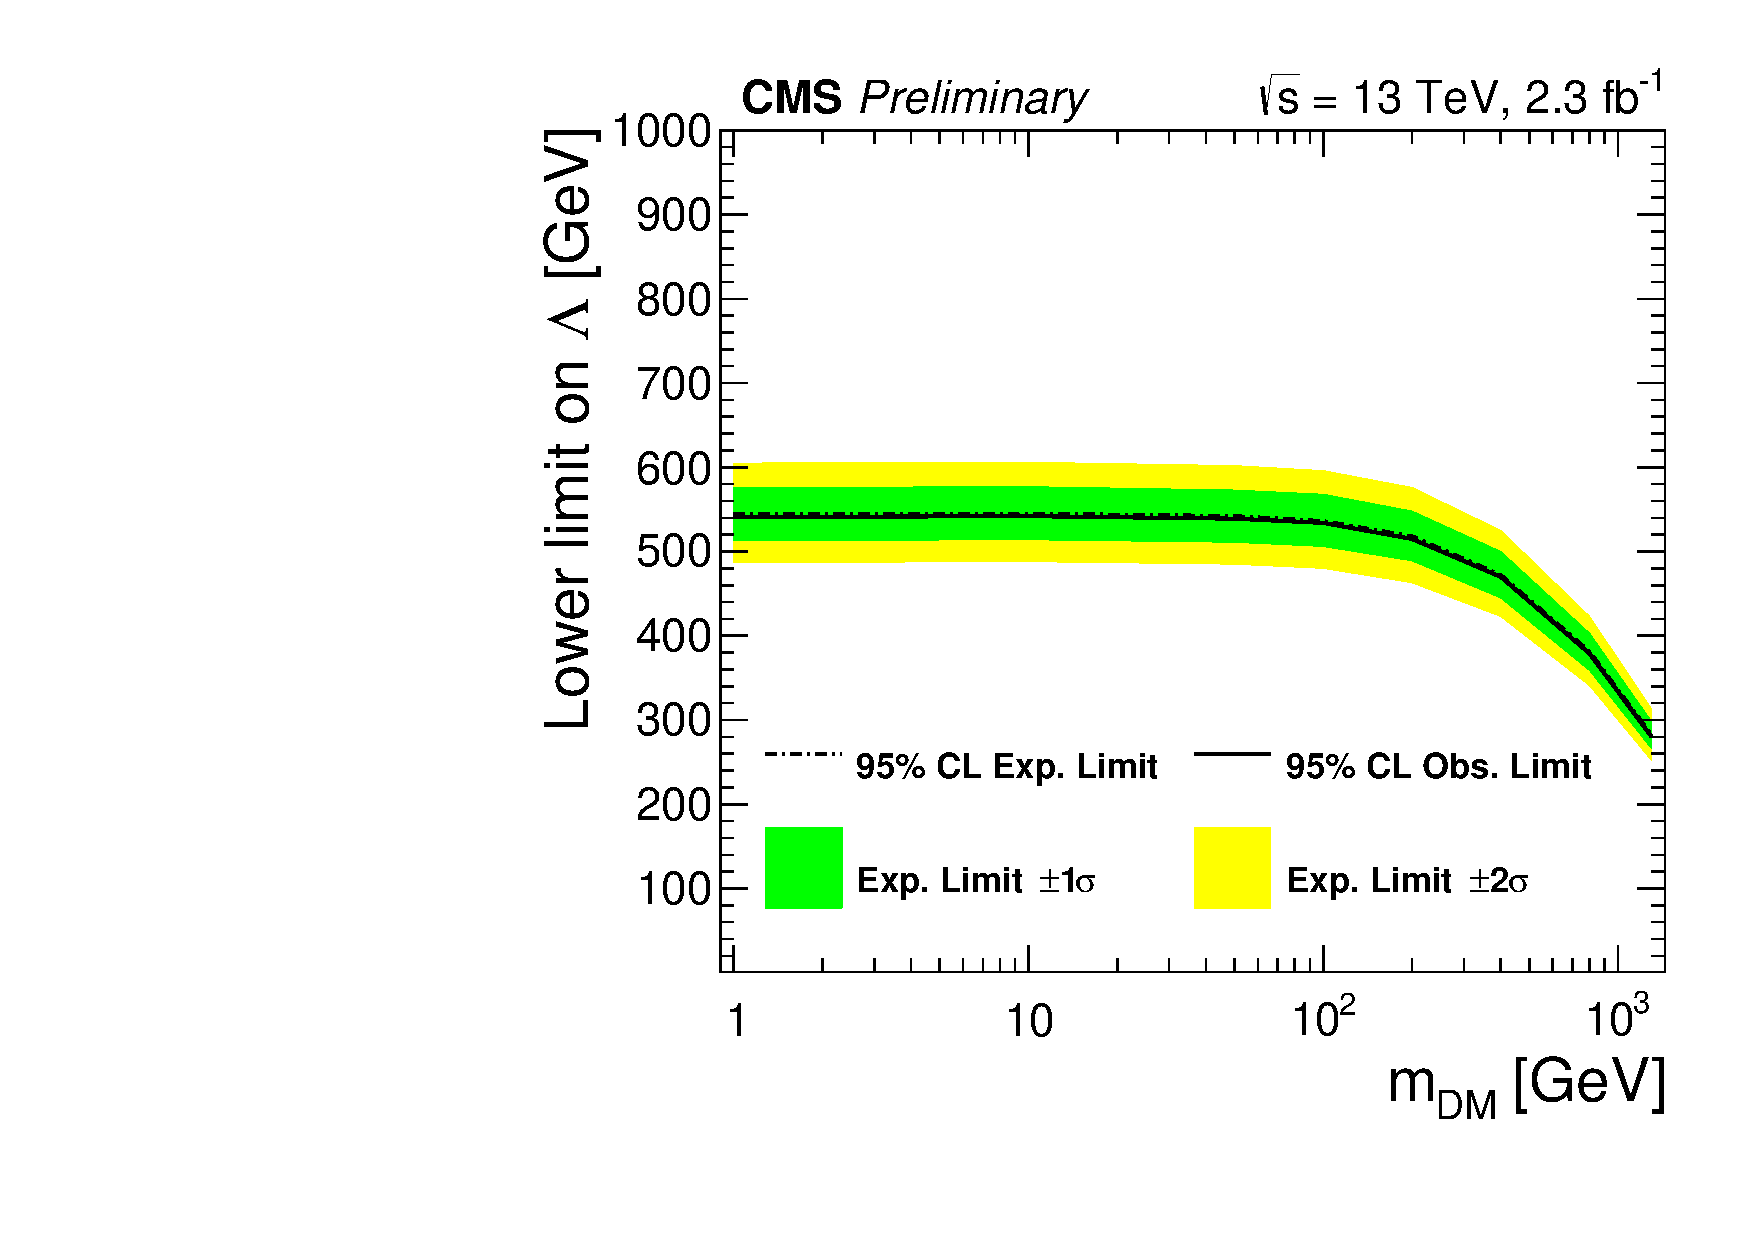
\includegraphics[width=0.4\textwidth]{pdfs/lgxc/fromb/EWK_lambda.pdf}
\end{center}
\end{figure}





